
\documentclass[%
    25pt, a1paper, portrait,%
    blockverticalspace=15pt,%
    colspace=15pt,%
    margin=0pt,%
    innermargin=20pt,%
]{tikzposter}

%%%%%%%%%%%%%%%%%%%%%%%%%%%%%%%%%%%%%%%%%%%%
% PACKAGES
%%%%%%%%%%%%%%%%%%%%%%%%%%%%%%%%%%%%%%%%%%%%

\usepackage[english]{babel}
\usepackage{amsmath, amsthm, amssymb, latexsym}
\usepackage[utf8]{inputenc}
\usepackage{etoolbox}
\usepackage{xparse}
\usepackage{subcaption}
\usepackage{blindtext}
\usepackage{geometry}
\usepackage{calculator}
\usepackage[thicklines]{cancel}
\usepackage{tikz}
\usetikzlibrary{positioning}
\usepackage[absolute, overlay]{textpos}

\usepackage{calculator}



\makeatletter

\NewDocumentCommand{\setFontSize}{m o m}{%
    \IfNoValueF{#2}{%
        \fontsize{#1}{#2}\selectfont#3%
    }{%
        % see https://texblog.org/2012/08/29/changing-the-font-size-in-latex/
        \MULTIPLY{#1}{1.2}{\setFont@baseline}%
        \fontsize{#1}{\setFont@baseline}\selectfont#3%
    }%
}

\NewDocumentCommand{\todo}{m}{%
    {\color{blue} #1}%
}

\NewDocumentCommand{\code}{m}{%
    \texttt{#1}%
}

% draw a square.
% param1: fill color red!50
% param2: border color (default to black)
\NewDocumentCommand{\drawFilledSquare}{m O{black}}{%
    \begin{tikzpicture}%
        \node [rectangle,draw={#2},fill={#1}] (m) at (0,0) {};%
    \end{tikzpicture}%
}

\NewDocumentCommand{\eg}{}{%
    e.g.,%
}

\NewDocumentCommand{\ie}{}{%
    i.e.,%
}

\NewDocumentCommand{\wrt}{}{%
    w.r.t.%
}

\NewDocumentEnvironment{coloredBlock}{m O{blue} O{white}}{%
\setbeamercolor{block title}{bg=#2, fg=#3}
    \begin{block}{#1}%
}{%
    \end{block}%
}

\NewDocumentCommand{\doublePlus}{}{%
    \ifmmode{+\!\!+}\else{$+\!\!+$}\fi%
}

\makeatother
\NewDocumentCommand{\CPD}{}{%
    \texttt{CPD}%
}

\NewDocumentCommand{\ALT}{}{%
    \texttt{ALT}%
}

\NewDocumentCommand{\AWA}{}{%
    \texttt{AWA$^*$}%
}

\NewDocumentCommand{\WA}{}{%
    \texttt{WA$^*$}%
}

\NewDocumentCommand{\A}{}{%
    \texttt{A$^*$}%
}

\NewDocumentCommand{\CPDSearch}{}{%
    \texttt{CPD-Search}%
}

\NewDocumentCommand{\anytimeCPDSearch}{}{%
    \texttt{Anytime CPD-Search}%
}


\NewDocumentCommand{\CPDPathName}{}{%
    \texttt{CPD}-Path%
}

\NewDocumentCommand{\CPDPathsName}{}{%
    \texttt{CPD}-Paths%
}

\NewDocumentCommand{\CPDPath}{m m}{%
    \texttt{CPD-Path}[#1, #2]%
}

\NewDocumentCommand{\CPDPathCostOriginal}{m m}{%
    \ifmmode{h_{CPD}[#1]}\else{$h_{CPD}[#1]$}\fi%
}

\NewDocumentCommand{\CPDPathCostNew}{m m}{%
    \ifmmode{h'_{CPD}[#1]}\else{$h'_{CPD}[#1]$}\fi%
}

\NewDocumentCommand{\pathOnGraph}{m m}{%
    path[#1, #2]%
}

%%%%%%%%%%%%%%%%%%%%%%%%%%%%%%%%%%%%%%%%%%%%
% TITLE
%%%%%%%%%%%%%%%%%%%%%%%%%%%%%%%%%%%%%%%%%%%%

\title{%
    Path Planning with CPD Heuristics%
}
\author{Massimo Bono$^1$, Alfonso E. Gerevini$^1$, Daniel D. Harabor$^2$, Peter J. Stuckey$^2$}
\date{\today}
\institute{%
    $^1$\setFontSize{42}{Dipartimento Di Ingegneria dell'Informazione, Università degli Studi di Brescia, Brescia, Italy}%
    \\%
    $^2$\setFontSize{42}{Faculty of Information Technology, Monash University, Melbourne, Australia}%
}

%%%%%%%%%%%%%%%%%%%%%%%%%%%%%%%%%%%%%%%%%%
% STYLE
%%%%%%%%%%%%%%%%%%%%%%%%%%%%%%%%%%%%%%%%%%

\definecolorpalette{customColorPalette}{%
    \definecolor{colorOne}{rgb}{0.2, 0.2, 0.6}%
    \definecolor{colorTwo}{rgb}{0.36, 0.54, 0.66}%
    \definecolor{colorThree}{rgb}{0.2, 0.2, 0.6}
}
\usetheme{Autumn}
\usecolorstyle[colorPalette=customColorPalette]{Germany}

%%%%%%%%%%%%%%%%%%%%%%%%%%%%%%%%%%%%%%%%%%
% configuration of tikzposter
%%%%%%%%%%%%%%%%%%%%%%%%%%%%%%%%%%%%%%%%%%

%remove logo https://tex.stackexchange.com/a/263278/145331
\tikzposterlatexaffectionproofoff

%%%%%%%%%%%%%%%%%%%%%%%%%%%%%%%%%%%%%%%%%%
% TEXPOS CONFIGURATION
%%%%%%%%%%%%%%%%%%%%%%%%%%%%%%%%%%%%%%%%%%

\setlength{\TPHorizModule}{1mm}
\setlength{\TPVertModule}{1mm}
\dimendef\prevdepth=0
%\textblockorigin{0mm}{0mm} % start everything near the top-left corner

%%%%%%%%%%%%%%%%%%%%%%%%%%%%%%%%%%%%%%%%%%
% TIKZ CONFIGURATION
%%%%%%%%%%%%%%%%%%%%%%%%%%%%%%%%%%%%%%%%%%

\tikzset{Vertex/.style={%
    shape=circle,%
    draw=blue!30,%
    fill=blue!15,%
    minimum size=10pt,%
    line width=4pt,%
    radius=1cm,%
    inner sep=3pt,%
    node distance=3.5cm,%
}}
\tikzset{StartVertex/.style={%
    shape=circle,%
    draw=blue!50,%
    fill=blue!30,%
    minimum size=10pt,%
    line width=7pt,%
    radius=1cm,%
    inner sep=3pt,%
    node distance=3.5cm,%
}}
\tikzset{TargetVertex/.style={%
    shape=circle,%
    draw=blue!50,%
    fill=blue!30,%
    minimum size=10pt,%
    line width=7pt,%
    radius=1cm,%
    inner sep=3pt,%
    node distance=3.5cm,%
}}
\tikzset{SearchNode/.style={%
    shape=circle,%
    draw=yellow!80,%
    fill=yellow!50,%
    minimum size=10pt,%
    line width=7pt,%
    radius=1cm,%
    inner sep=3pt,%
    node distance=3.5cm,%
}}
\tikzset{NormalEdge/.style={%
    -.,
    line width=2pt,%
}}
\tikzset{EdgePath/.style={%
    ->,%
    line width=5pt,%
}}
\tikzset{HPath/.style={%
    ->,%
    dashed,%
    line width=5pt,%
}}
\NewDocumentCommand{\edgeLabel}{s m}{%
    \IfBooleanTF{#1}{%
        \Large{\textbf{\color{red}#2}}%
    }{%
        \Large{\textbf{#2}}%
    }%
}

%%%%%%%%%%%%%%%%%%%%%%%%%%%%%%%%%%%%%%%%%%%%
% DOCUMENT
%%%%%%%%%%%%%%%%%%%%%%%%%%%%%%%%%%%%%%%%%%%%

\begin{document}

    \maketitle

    \begin{textblock}{45}[0.5, 0.5](55,30)
        
\includegraphics[width=45mm]{src/images/unibs-onlylogo3}
    \end{textblock}

    \begin{textblock}{45}[0.5, 0.5](539,30)
        
\includegraphics[width=45mm]{src/images/monash-onlylogo2}
    \end{textblock}

    \block{Abstract}{%
        Compressed Path Databases (CPDs) are a leading technique for optimal pathfinding in graphs with static edge costs. In this work we investigate CPDs as admissible heuristic functions and we apply them in two distinct settings: problems where the graph is subject to dynamically changing costs, and anytime settings where deliberation time is limited. Conventional heuristics derive cost-to- go estimates by reasoning about a tentative and usually infeasible path, from the current node to the target. CPD-based heuristics derive cost-to-go estimates by computing a concrete and usually feasible path. We exploit such paths to bound the optimal solution, not just from below but also from above. We demonstrate the benefit of this approach in a range of experiments on standard gridmaps and in comparison to Landmarks, a popular alternative also developed for searching in explicit state-spaces.
    }

    \block{Problem}{%
        \begin{minipage}{0.31\textwidth}%
            \centering%
            \textbf{Original map}%
            \medskip\medskip\medskip

            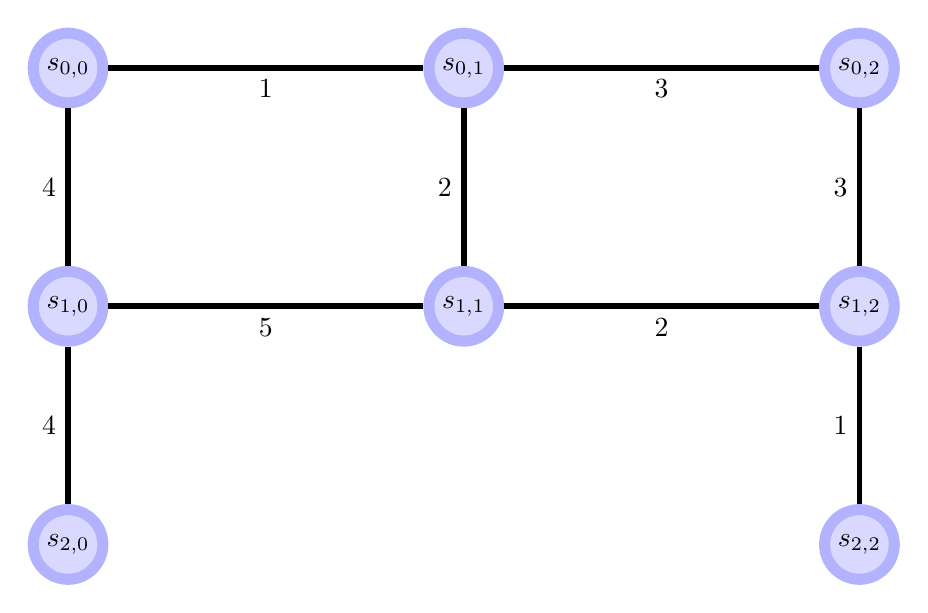
\begin{tikzpicture}
    \node[Vertex] (v00) at (0,0) {$s_{0,0}$};
    \node[Vertex, right=4.0cm of v00] (v01) {$s_{0,1}$};
    \node[Vertex, right=4.0cm of v01] (v02) {$s_{0,2}$};
    \node[Vertex, below=2.0cm of v00] (v10) {$s_{1,0}$};
    \node[Vertex, right=4.0cm of v10] (v11) {$s_{1,1}$};
    \node[Vertex, right=4.0cm of v11] (v12) {$s_{1,2}$};
    \node[Vertex, below=2.0cm of v10] (v20) {$s_{2,0}$};
    \node[Vertex, below=2.0cm of v12] (v22) {$s_{2,2}$};

    \path (v00) edge[NormalEdge] node[below]{\edgeLabel{1}} (v01);
    \path (v01) edge[NormalEdge] node[below]{\edgeLabel{3}} (v02);
    \path (v10) edge[NormalEdge] node[below]{\edgeLabel{5}} (v11);
    \path (v11) edge[NormalEdge] node[below]{\edgeLabel{2}} (v12);
    \path (v00) edge[NormalEdge] node[left]{\edgeLabel{4}} (v10);
    \path (v10) edge[NormalEdge] node[left]{\edgeLabel{4}} (v20);
    \path (v01) edge[NormalEdge] node[left]{\edgeLabel{2}} (v11);
    \path (v02) edge[NormalEdge] node[left]{\edgeLabel{3}} (v12);
    \path (v12) edge[NormalEdge] node[left]{\edgeLabel{1}} (v22);
\end{tikzpicture}
        \end{minipage}%
        \begin{minipage}{0.31\textwidth}
            \centering
            \textbf{Solution of query $\mathbf{q = (s_{0,0}, s_{2,2})}$}
            \medskip\medskip\medskip
            
            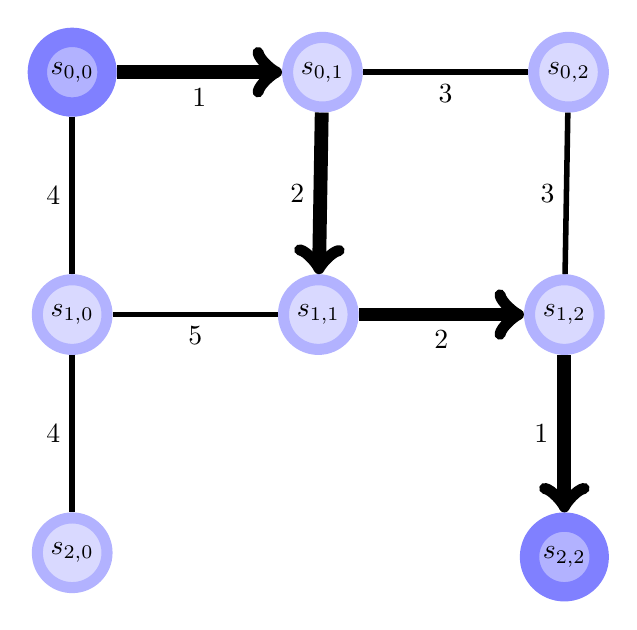
\begin{tikzpicture}
    \node[StartVertex] (v00) at (0,0) {$s_{0,0}$};
    \node[Vertex, right=2.1cm of v00] (v01) {$s_{0,1}$};
    \node[Vertex, right=2.1cm of v01] (v02) {$s_{0,2}$};
    \node[Vertex, below=2.0cm of v00] (v10) {$s_{1,0}$};
    \node[Vertex, right=2.1cm of v10] (v11) {$s_{1,1}$};
    \node[Vertex, right=2.1cm of v11] (v12) {$s_{1,2}$};
    \node[Vertex, below=2.0cm of v10] (v20) {$s_{2,0}$};
    \node[TargetVertex, below=2.0cm of v12] (v22) {$s_{2,2}$};

    \path (v00) edge[EdgePath] node[below]{\edgeLabel{1}} (v01);
    \path (v01) edge[NormalEdge] node[below]{\edgeLabel{3}} (v02);
    \path (v10) edge[NormalEdge] node[below]{\edgeLabel{5}} (v11);
    \path (v11) edge[EdgePath] node[below]{\edgeLabel{2}} (v12);
    \path (v00) edge[NormalEdge] node[left]{\edgeLabel{4}} (v10);
    \path (v10) edge[NormalEdge] node[left]{\edgeLabel{4}} (v20);
    \path (v01) edge[EdgePath] node[left]{\edgeLabel{2}} (v11);
    \path (v02) edge[NormalEdge] node[left]{\edgeLabel{3}} (v12);
    \path (v12) edge[EdgePath] node[left]{\edgeLabel{1}} (v22);
\end{tikzpicture}
        \end{minipage}%
        \begin{minipage}{0.31\textwidth}
            \centering
            \textbf{Problem: compute solution of $\mathbf{q}$ over map with \textit{perturbations}?}
            \medskip\medskip\medskip
            
            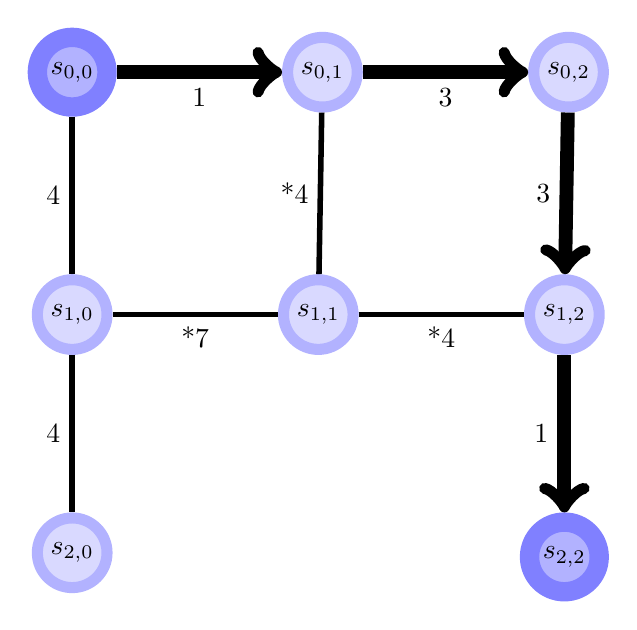
\begin{tikzpicture}
    \node[StartVertex] (v00) at (0,0) {$s_{0,0}$};
    \node[Vertex, right=2.1cm of v00] (v01) {$s_{0,1}$};
    \node[Vertex, right=2.1cm of v01] (v02) {$s_{0,2}$};
    \node[Vertex, below=2.0cm of v00] (v10) {$s_{1,0}$};
    \node[Vertex, right=2.1cm of v10] (v11) {$s_{1,1}$};
    \node[Vertex, right=2.1cm of v11] (v12) {$s_{1,2}$};
    \node[Vertex, below=2.0cm of v10] (v20) {$s_{2,0}$};
    \node[TargetVertex, below=2.0cm of v12] (v22) {$s_{2,2}$};

    \path (v00) edge[EdgePath] node[below]{\edgeLabel{1}} (v01);
    \path (v01) edge[EdgePath] node[below]{\edgeLabel{3}} (v02);
    \path (v10) edge[NormalEdge] node[below]{\edgeLabel*{7}} (v11);
    \path (v11) edge[NormalEdge] node[below]{\edgeLabel*{4}} (v12);
    \path (v00) edge[NormalEdge] node[left]{\edgeLabel{4}} (v10);
    \path (v10) edge[NormalEdge] node[left]{\edgeLabel{4}} (v20);
    \path (v01) edge[NormalEdge] node[left]{\edgeLabel*{4}} (v11);
    \path (v02) edge[EdgePath] node[left]{\edgeLabel{3}} (v12);
    \path (v12) edge[EdgePath] node[left]{\edgeLabel{1}} (v22);
\end{tikzpicture}
        \end{minipage}%
    }

    \block{\CPDSearch{} $\Rightarrow$ Exploit \CPDPathsName{} in an \A{} variant}{%
        \begin{minipage}{0.26\textwidth}
                \begin{tabular}{c|cccccccc}
                st          & $s_{0,0}$ & $s_{0,1}$ & $s_{0,2}$ &$s_{1,0}$ &$s_{1,1}$ &$s_{1,2}$ &$s_{2,0}$ &$s_{2,2}$ \\ \hline
                $s_{0,0}$   & * & a & a & e & a & a & e & a \\
                $s_{0,1}$   & a & * & b & a & g & g & a & g \\
                $s_{0,2}$   & b & b & * & b & b & h & b & h \\
                $s_{1,0}$   & e & e & e & * & c & c & f & c \\
                $s_{1,1}$   & g & g & g & c & * & d & c & d \\
                $s_{1,2}$   & d & d & h & d & d & * & d & i \\
                $s_{2,0}$   & f & f & f & f & f & f & * & f \\
                $s_{2,2}$   & i & i & i & i & i & i & i & * \\
                \end{tabular}
        \end{minipage}\quad%
        \begin{minipage}{0.23\textwidth}
            \centering
            \textbf{Admissible heuristic}
            \medskip\medskip\medskip

            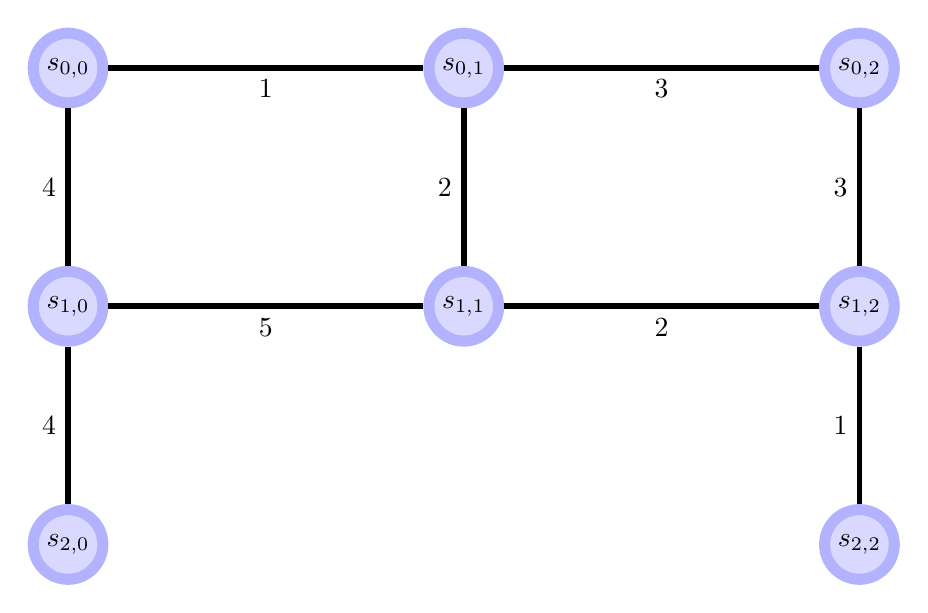
\begin{tikzpicture}
    \node[Vertex] (v00) at (0,0) {$s_{0,0}$};
    \node[Vertex, right=4.0cm of v00] (v01) {$s_{0,1}$};
    \node[Vertex, right=4.0cm of v01] (v02) {$s_{0,2}$};
    \node[Vertex, below=2.0cm of v00] (v10) {$s_{1,0}$};
    \node[Vertex, right=4.0cm of v10] (v11) {$s_{1,1}$};
    \node[Vertex, right=4.0cm of v11] (v12) {$s_{1,2}$};
    \node[Vertex, below=2.0cm of v10] (v20) {$s_{2,0}$};
    \node[Vertex, below=2.0cm of v12] (v22) {$s_{2,2}$};

    \path (v00) edge[NormalEdge] node[below]{\edgeLabel{1}} (v01);
    \path (v01) edge[NormalEdge] node[below]{\edgeLabel{3}} (v02);
    \path (v10) edge[NormalEdge] node[below]{\edgeLabel{5}} (v11);
    \path (v11) edge[NormalEdge] node[below]{\edgeLabel{2}} (v12);
    \path (v00) edge[NormalEdge] node[left]{\edgeLabel{4}} (v10);
    \path (v10) edge[NormalEdge] node[left]{\edgeLabel{4}} (v20);
    \path (v01) edge[NormalEdge] node[left]{\edgeLabel{2}} (v11);
    \path (v02) edge[NormalEdge] node[left]{\edgeLabel{3}} (v12);
    \path (v12) edge[NormalEdge] node[left]{\edgeLabel{1}} (v22);
\end{tikzpicture}            
        \end{minipage}%
        \begin{minipage}{0.23\textwidth}
            \centering
            \textbf{Early Termination}
            \medskip\medskip\medskip

            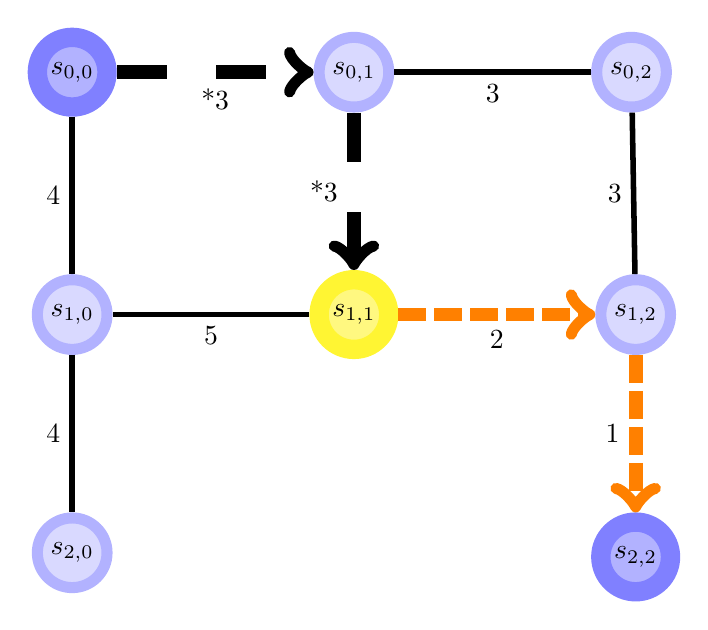
\begin{tikzpicture}
    \node[StartVertex] (v00) at (0,0) {$s_{0,0}$};
    \node[Vertex, right=2.5cm of v00] (v01) {$s_{0,1}$};
    \node[Vertex, right=2.5cm of v01] (v02) {$s_{0,2}$};
    \node[Vertex, below=2.0cm of v00] (v10) {$s_{1,0}$};
    \node[SearchNode, right=2.5cm of v10] (v11) {$s_{1,1}$};
    \node[Vertex, right=2.5cm of v11] (v12) {$s_{1,2}$};
    \node[Vertex, below=2.0cm of v10] (v20) {$s_{2,0}$};
    \node[TargetVertex, below=2.0cm of v12] (v22) {$s_{2,2}$};

    \path (v00) edge[EdgePath, dash pattern=on 18pt off 18pt] node[below]{\edgeLabel*{3}} (v01);
    \path (v01) edge[NormalEdge] node[below]{\edgeLabel{3}} (v02);
    \path (v10) edge[NormalEdge] node[below]{\edgeLabel{5}} (v11);
    \path (v11) edge[EdgePath, EdgePath, dash pattern=on 10pt off 3pt, draw=orange] node[below]{\edgeLabel{2}} (v12);
    \path (v00) edge[NormalEdge] node[left]{\edgeLabel{4}} (v10);
    \path (v10) edge[NormalEdge] node[left]{\edgeLabel{4}} (v20);
    \path (v01) edge[EdgePath, dash pattern=on 18pt off 18pt] node[left]{\edgeLabel*{3}} (v11);
    \path (v02) edge[NormalEdge] node[left]{\edgeLabel{3}} (v12);
    \path (v12) edge[EdgePath, EdgePath, dash pattern=on 10pt off 3pt, draw=orange] node[left]{\edgeLabel{1}} (v22);
\end{tikzpicture}            
        \end{minipage}%
        \begin{minipage}{0.23\textwidth}
            \centering
            \textbf{Obtain solution bounds}
            \medskip\medskip\medskip

            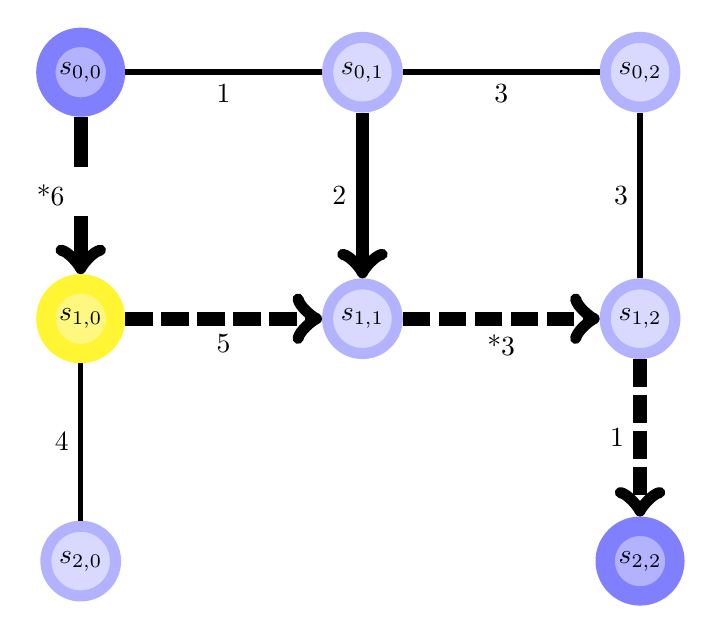
\begin{tikzpicture}
    \node[StartVertex] (v00) at (0,0) {$s_{0,0}$};
    \node[Vertex, right=2.5cm of v00] (v01) {$s_{0,1}$};
    \node[Vertex, right=2.5cm of v01] (v02) {$s_{0,2}$};
    \node[SearchNode, below=2.0cm of v00] (v10) {$s_{1,0}$};
    \node[Vertex, right=2.5cm of v10] (v11) {$s_{1,1}$};
    \node[Vertex, right=2.5cm of v11] (v12) {$s_{1,2}$};
    \node[Vertex, below=2.0cm of v10] (v20) {$s_{2,0}$};
    \node[TargetVertex, below=2.0cm of v12] (v22) {$s_{2,2}$};

    \path (v00) edge[NormalEdge] node[below]{\edgeLabel{1}} (v01);
    \path (v01) edge[NormalEdge] node[below]{\edgeLabel{3}} (v02);
    \path (v10) edge[EdgePath,dash pattern=on 10pt off 3pt] node[below]{\edgeLabel{5}} (v11);
    \path (v11) edge[EdgePath,dash pattern=on 10pt off 3pt] node[below]{\edgeLabel*{3}} (v12);
    \path (v00) edge[EdgePath, dash pattern=on 18pt off 18pt] node[left]{\edgeLabel*{6}} (v10);
    \path (v10) edge[NormalEdge] node[left]{\edgeLabel{4}} (v20);
    \path (v01) edge[EdgePath] node[left]{\edgeLabel{2}} (v11);
    \path (v02) edge[NormalEdge] node[left]{\edgeLabel{3}} (v12);
    \path (v12) edge[EdgePath,dash pattern=on 10pt off 3pt] node[left]{\edgeLabel{1}} (v22);
\end{tikzpicture}            
        \end{minipage}

    }

    \begin{columns}
        \column{0.630}{%
            \block{Optimal scenario}{%
                \begin{minipage}{0.5\linewidth}
                    \centering
                    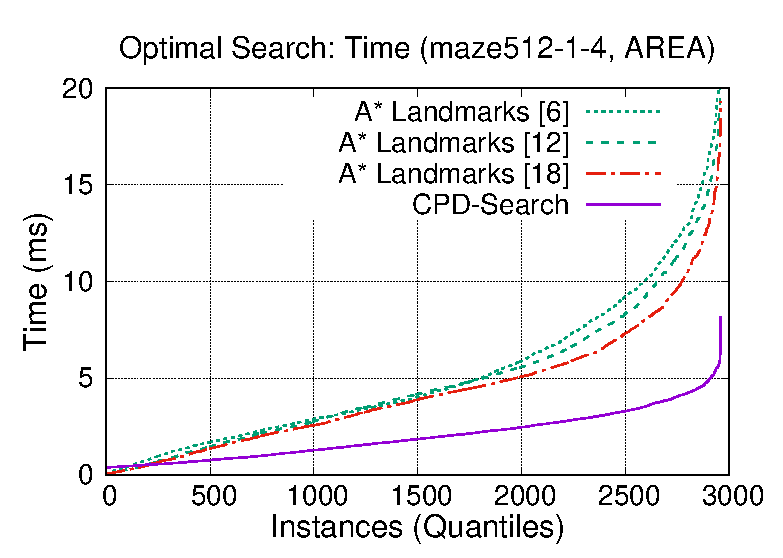
\includegraphics[width=1.0\linewidth]{src/images/maze512-1-4}
                \end{minipage}\hfill%
                \begin{minipage}{0.5\linewidth}
                    \centering
                    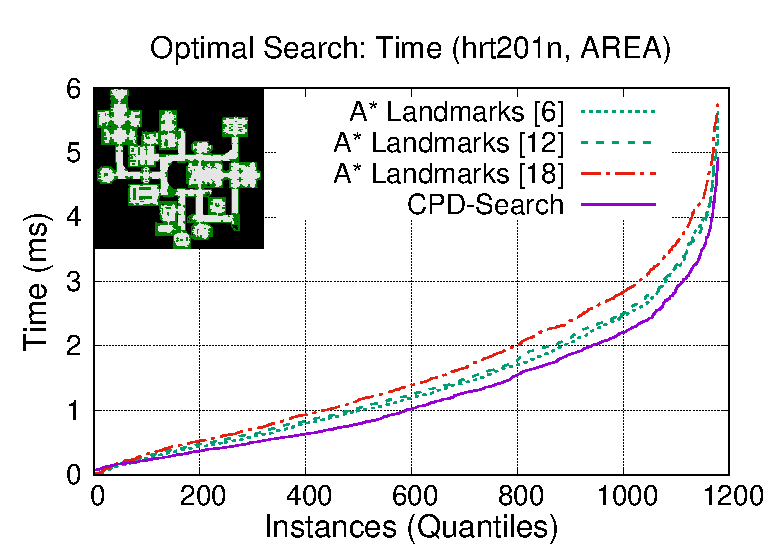
\includegraphics[width=1.0\linewidth]{src/images/hrt201n}
                \end{minipage}
            }
        }%
        \column{0.36}{%
            \block{Anytime scenario}{%
                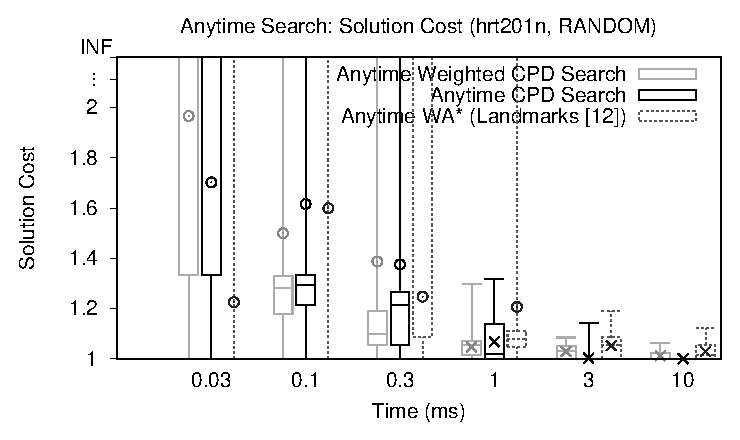
\includegraphics[width=1.0\linewidth]{src/images/anytime}
                %add space to fill everything
                \phantom{x}
            }
        }
    \end{columns}
    
\end{document}